\documentclass[pdf]{beamer}
\mode<presentation>{\usecolortheme{crane}}
%% preamble
\title{Simulation of CSE Lab Cluster}
\subtitle{CS633 2018-19-II Course Project}
\author{Yash Srivastav (150839)}
\date{March 12, 2018}

% \AtBeginSection[]
% {
%   \begin{frame}{Table of Contents}
%     \tableofcontents[currentsection]
%   \end{frame}
% }

\AtBeginSubsection[]
{
  \begin{frame}{Table of Contents}
    \tableofcontents[currentsubsection]
  \end{frame}
}

\begin{document}
%% title frame
\begin{frame}
  \titlepage
\end{frame}
%% normal frame
\section{Introduction}
\subsection{Description}
\begin{frame}{CSE Lab Cluster}
  \begin{itemize}
    \item<1-> Consists of $\sim{} 30$ PCs connected over LAN
    \item<2-> Hostfiles used for MPI programs usually don't take topology or
      placement into account
    \item<3-> We want to simulate the running of an MPI program on this cluster
      and predict time taken for communications
    \item<4-> Would enable simulating under different hostfiles and use it to
      decide upon which one to use
  \end{itemize}
\end{frame}
\begin{frame}{CSE Lab Cluster Topology}
  \begin{figure}[ht]
    \begin{center}
      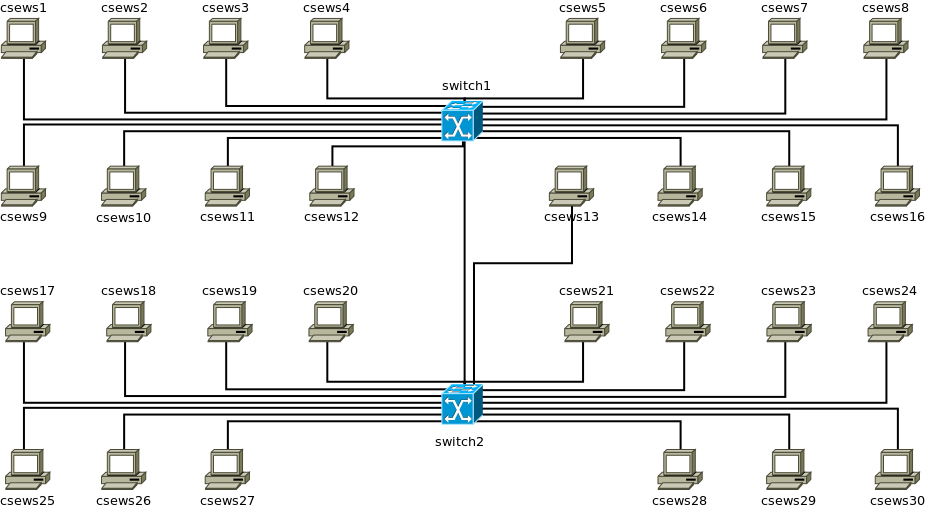
\includegraphics[width=\textwidth]{topology}
    \end{center}
  \end{figure}
  \begin{itemize}
    \item \texttt{csews13} is on different switch from remaining \texttt{csews1-16}
  \end{itemize}
\end{frame}
\subsection{Related Work}
\begin{frame}{Related Research Papers}
  \begin{itemize}
    \item MPI-NeTSim: A network simulation module for MPI \cite{netsim}
    \item Simulation of MPI Applications with Time-independent Traces
      \cite{time-independent-trace-sim}
    \item Single Node On-Line Simulation of MPI Applications with SMPI
      \cite{smpi-online}
    \item Toward Better Simulation of MPI Applications on Ethernet/TCP
      Networks \cite{better-sim-ethernet}
    \item Simulating MPI applications: the SMPI approach \cite{smpi}
  \end{itemize}
\end{frame}
\subsection{Approach and Challenges}
\begin{frame}{Initial Approach (without referring to related work)}
  \begin{itemize}
    \item<1-> Obtain event traces for the target MPI program by running it on a
      host machine with the required number of processes.
    \item<2-> Separate all communications into time slots which can be simulated
      as occurring concurrently.
    \item<3-> Using the knowledge of the network topology and a given hostfile,
      perform simulation based on the trace obtained in a network simulation
      framework.
    \item<4-> Report the expected time taken for communications and congestion
      points/links, if any.
  \end{itemize}
\end{frame}
\begin{frame}{Sample Time Slotting}
  \begin{figure}[ht]
    \begin{center}
      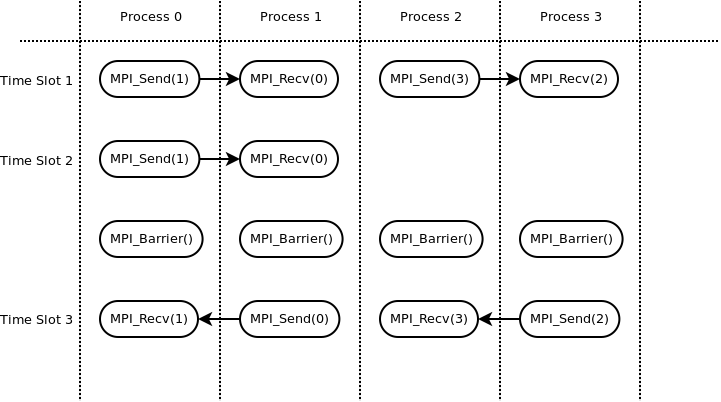
\includegraphics[width=\textwidth]{time-slots}
    \end{center}
  \end{figure}
\end{frame}
\begin{frame}{Drawbacks/Challenges}
  \begin{itemize}
    \item<1-> Doesn't take into account the computation period in-between
      communications.
    \item<2-> Even if we were to take computation period into account, there is
      no reliable way of getting it on an over-subscribed host as
      \texttt{MPI\_WTime} returns values from fixed past time and does not take
      process scheduling into account.
    \item<3-> Also computation time would come out to be different for different
      ranked processes based on scheduling / other loads on the CPU / etc even
      if they were running the same set of instructions.
  \end{itemize}
\end{frame}
\begin{frame}{Refined Approach (inspired by related work)}
  \begin{itemize}
    \item<1-> Obtain time-independent event traces for the target MPI program
      similar to \cite{time-independent-trace-sim}.
    \item<2-> The above gives us bytes transferred (for communications) and
      number of instructions executed (for computations).
    \item<3-> Using the knowledge of the network topology and a given hostfile,
      perform simulation based on the trace obtained in an event-based network
      simulation framework.
    \item<4-> Report the expected time taken for communications and congestion
      points/links, if any.
  \end{itemize}
\end{frame}
\begin{frame}{Sample Trace}
  \begin{figure}[ht]
    \begin{center}
      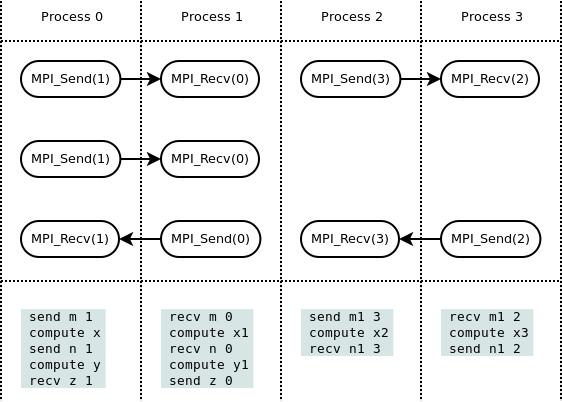
\includegraphics[width=\textwidth]{ti-trace}
    \end{center}
  \end{figure}
\end{frame}
\begin{frame}{Obtaining Event Traces}
  \begin{itemize}
    \item<1-> We use the \texttt{PMPI\_} interface exposed by nearly all MPI
      implementations inorder to override calls to \texttt{MPI\_} functions with
      custom code. This allows us to log calls.
    \item<2-> We also use the \textbf{Performance Application Programming
        Interface (PAPI)} \cite{papi} in order to measure CPU cycles /
      instructions between 2 MPI calls (computation). Since PAPI counters are
      thread specific, this approach is valid on over-subscribed MPI executions
      as well.
    \item<3-> At the end of an invocation of an MPI call, we note down the value
      of the performance counter. At the start of the next MPI call, the
      difference between the counter value is the computation.
  \end{itemize}
  % Challenges:
\end{frame}
\begin{frame}{Obtaining Event Traces - Challenges / Drawbacks}
  \begin{itemize}
    \item<1-> In order to collect the traces on a single machine, the machine
      should have enough memory for all the processes.
    \item<2-> The trace size grows pretty large for non-trivial applications.
    \item<3-> This would also log internal \texttt{MPI\_Send} and
      \texttt{MPI\_Recv} used by MPI Collectives. For that, we could set a flag
      before a collective call and reset it after the call.
    \item<4-> The tracing machine should have the same processor architecture
      as the CSE lab cluster. Since our tracer would run on one of the lab
      machines, it is not an issue.
    \item<5-> The computation time during MPI calls is ignored by our simulation
      but its ok because its expected for it be negligible compared to the
      communication time over the network.
  \end{itemize}
\end{frame}
\begin{frame}{Offline Simulation}
  \begin{itemize}
    \item<1-> Using the information collected by the traces and a provided
      hostfile, we could generate an event stream for each node on the cluster.
    \item<2-> The above event stream would be fed into an event-based network
      simulator like ns3 which has all the hosts configured as per the cse lab
      cluster topology.
    \item<3-> This should give us the expected time for each event and also
      allow us to identify limiting link contentions.
    \item<4-> \textbf{NOTE:} The ns3 framework needs a little more exploration
      to finalize this part.
  \end{itemize}
\end{frame}
\section{Targets}
\subsection{``Must-Have''s}
\begin{frame}{MPI Calls}
  The final simulator should be able to simulate/handle the following synchronous
  MPI calls with accurate algorithms as used in default \texttt{MPICH v3.2.1}:
  \begin{itemize}
    \item \texttt{MPI\_Send}
    \item \texttt{MPI\_Recv}
    \item \texttt{MPI\_Broadcast}
    \item \texttt{MPI\_Reduce}
    \item \texttt{MPI\_Scatter}
    \item \texttt{MPI\_Allreduce}
    \item \texttt{MPI\_Alltoall}
    \item \texttt{MPI\_Gather}
    \item \texttt{MPI\_Allgather}
    \item \texttt{MPI\_Barrier}
  \end{itemize}
\end{frame}
\begin{frame}[fragile]
  \frametitle{Simulation Semantics}
  This is how the final \textbf{Sim}ulated \textbf{MPI} should be invoked:
\begin{semiverbatim}
\$ simpicc \$FLAGS -o prog.x prog.c
\$ simpirun -f hostfile -np 32 prog.x
\end{semiverbatim}
  \texttt{hostfile} should contain only hosts on the cse lab cluster with
  hostnames as \texttt{csews1}, etc.
\end{frame}
\subsection{``Maybe''s}
\begin{frame}{MPI Calls}
  The final simulator may be able to simulate/handle the following MPI calls:
  \begin{itemize}
    \item Async variants and associated calls like \texttt{MPI\_Wait}
    \item Vector variants (like \texttt{MPI\_Allgatherv})
  \end{itemize}
\end{frame}
\begin{frame}[fragile]
  \frametitle{Simulation Semantics}
  This is how the final \textbf{Sim}ulated \textbf{MPI} may be invoked (I'm not
  sure if this is possible):
\begin{semiverbatim}
\$ export LD_PRELOAD=/path/to/simpilib/
\$ simpirun -f hostfile -np 32 prog.x
\end{semiverbatim}
  This would allow us to simulate precompiled binaries without modifying the
  makefile or recompiling.
\end{frame}
\begin{frame}{Misc Targets}
  \begin{itemize}
    \item<1-> Optimized tracefile size by using better binary formats like
      protobuf for trace storage.
    \item<2-> Proper \texttt{autotools} based installation setup for
      \texttt{simpi}.
  \end{itemize}
\end{frame}
\subsection{Future Possibilities}
\begin{frame}{Future Possibilities}
  Apart from the maybes described earlier, there are quite a few improvements
  which could be made:
  \begin{itemize}
    \item Distributed trace collection: The trace collection itself could be run
      parallelly on multiple machines for faster trace collection and simulation.
    \item Including / Predicting cpu cycles for the communication algorithm
      itself.
    \item Packet level simulation which is harder to get right.
  \end{itemize}
\end{frame}
\section{Current Progress}
\begin{frame}{Trace Generation}
  \begin{itemize}
    \item<1-> The current implementation of libsimpi can be used to generate traces for
      \texttt{MPI\_Send} and \texttt{MPI\_Recv}.
    \item<2-> Extending to others should not be difficult.
    \item<3-> Next target is to obtain computation count/cycles.
  \end{itemize}
\end{frame}
\begin{frame}[fragile]
  \frametitle{Sample \texttt{MPI\_Send} \texttt{PMPI} callback}
\begin{semiverbatim}
int MPI_Send(const void *buffer, int count,
             MPI_Datatype datatype, int dest,
             int tag, MPI_Comm comm) \{
  int size;
  int result = PMPI_Send(buffer, count,
                 datatype, dest, tag, comm);
  PMPI_Type_size(datatype, &size);
  fprintf(stderr, "[%d] send %d to %d\\n",
    rank, count * size, dest);
  return result;
\}
\end{semiverbatim}
\end{frame}
\begin{frame}[fragile]
  \frametitle{Sample Trace}
\begin{semiverbatim}
$ mpicc -g -O3 -profile=simpi asgn1-1.o -o asgn1-1.x  # link against libsimpi
$ mpirun -np 16 ./asgn1-1.x 1 > /dev/null  # discard stdout
[0] send 1024 to 1
[1] recv 1024 from 0
[2] send 1024 to 3
[3] recv 1024 from 2
[4] send 1024 to 5
[5] recv 1024 from 4
[6] send 1024 to 7
[7] recv 1024 from 6
[8] send 1024 to 9
[9] recv 1024 from 8
[10] send 1024 to 11
[11] recv 1024 from 10
[12] send 1024 to 13
[14] send 1024 to 15
[13] recv 1024 from 12
[15] recv 1024 from 14
\end{semiverbatim}
\end{frame}
\section{Conclusion}
\begin{frame}[c]
  \begin{center}
    \Huge Thank You!\\ \vspace{2mm}
    \tiny ``So long and thanks for all the fish.''  -- Douglas Adams
  \end{center}
\end{frame}
\subsection{References}
\begin{frame}[allowframebreaks]
  \frametitle{References}
  \bibliographystyle{amsalpha}
  \bibliography{progress}
\end{frame}

\end{document}
